

\section{Experiment Design}



\subsection{Robot Setup}
To evaluate our methodology, experiment is conducted on the Ant robot in PyBullet simulation \cite{PyBullet} (see Fig \ref{Ant_robot}). 
This robot has 8 degrees of freedom (2 for each leg) corresponding to 8 motors powering its motion.
Note that the joints connecting the body and each leg can only rotate horizontally, meaning that the four thighs (the part of each leg directly attached to the body) are always on the same plane.
Hence, the Ant robot cannot lift up its leg to walk like real animals.
The motors employ PID positional control, where the torque is given by:
\begin{equation}
\tau = K_p \theta_e + K_i \int \theta_e(t) dt + K_d \frac{d \theta_e}{dt}
\label{PID}
\end{equation}
where $\theta_e = \theta_t - \theta$ ($\theta_t$ is the positional target).
In PyBullet, the maximum torque is $\pm 1$. 
For the motors on the body, $K_p$ is set to be 1.43 and $K_d$ is set to be 0.072.
For the motors on the knees, $K_p$ is 1.637 and $K_d$ is 0.082.
For all motors, $K_i$ is set to zero for simplicity. 
\begin{figure}[h]
\centering
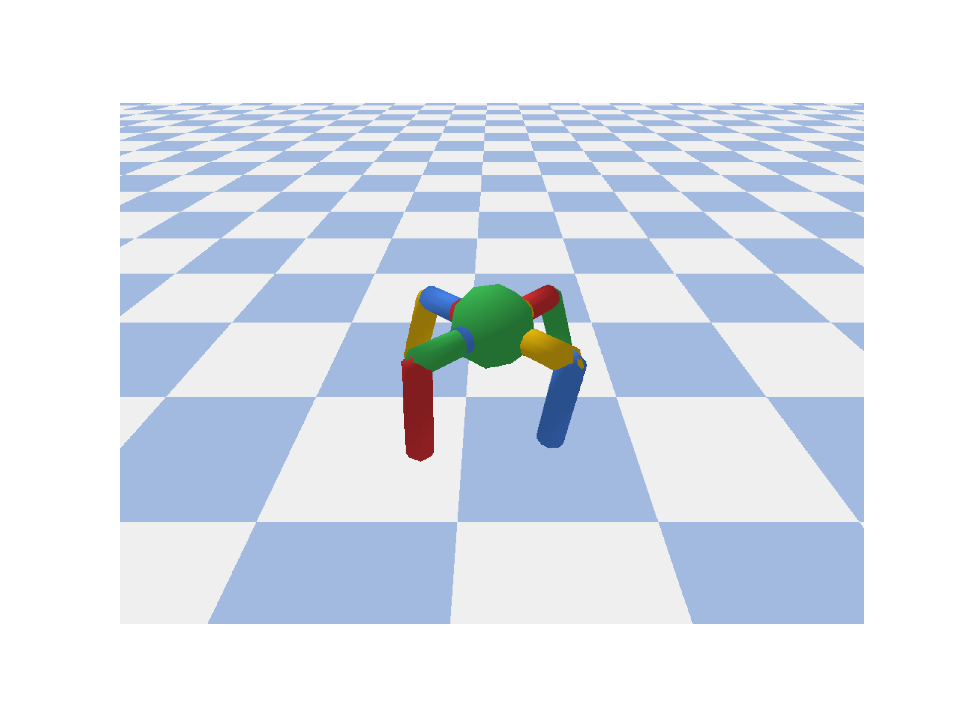
\includegraphics[width=0.45\textwidth]{intact_robot.pdf}
\caption{The Ant robot in PyBullet simulation. 
The four motors mounted on the body can rotate from $-40^{\circ}$ to $40^{\circ}$. The knee flexion angle for each leg ranges from 
$30^{\circ}$ to $100^{\circ}$.
}
\label{Ant_robot}
\end{figure}


Like in RTE, we use a periodic controller for the robot.
The period is set to 1 second, which corresponds to 100 time-steps in simulation.
The targets within each period is parametrized in the same way as in \cite{cully2015robots}.
The target of each motor is a smoothed squared wave (see Fig \ref{targets}) governed by three parameters: amplitude $\alpha$, phase $\phi$ and duty cycle $\tau$.
All the three parameters range from 0 to 1.
The duty cycle stands for the proportion of time in one period that the squared wave is in its high state.
This squared wave is then smoothed by a Gaussian kernel to remove rapid changes.
In each time-step of the simulation, we give each motor the corresponding positional target, which will then be converted into torques via PID.
Thus, each controller is parametrized by a vector of 24 dimensions, which is hence defined to be the genotype of this controller.
%
%
\begin{figure}[H]
\centering
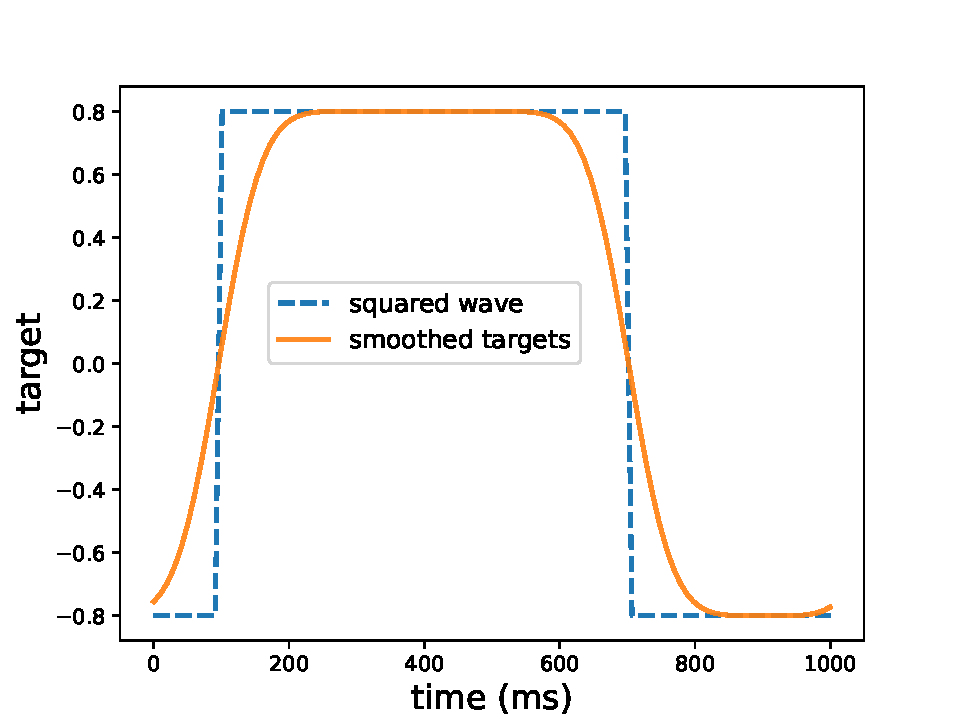
\includegraphics[width=0.45\textwidth]{targets.pdf}
\caption{The periodic motor targets corresponding to $\alpha = 0.8$, $\phi=100$ ms and $\tau=0.6$.
The squared wave is smoothed by a Gaussian kernel with $\sigma = 100$ ms.
}
\label{targets}
\end{figure}


In this paper, we consider three sources of distortions: friction, payload and damages to the legs of the robot.
To collect the distortions as the basis for the prior mean function, we need to model these sources in simulation.
Different frictions can be easily achieved by changing the simulation settings.
Leg damages are modelled by giving a fixed positional target to the motor mounted on the knee.
This fixed target overwrites the command of the controller, so that the damaged leg is always in the upper position (see Fig \ref{damaged_robot}).
However, for unknown reasons, changing the mass of the robot do not affect the dynamics in simulation. 
Hence, we take an alternative approach by discounting the torque to model the payload.
%
%
\begin{figure}[h]
\centering
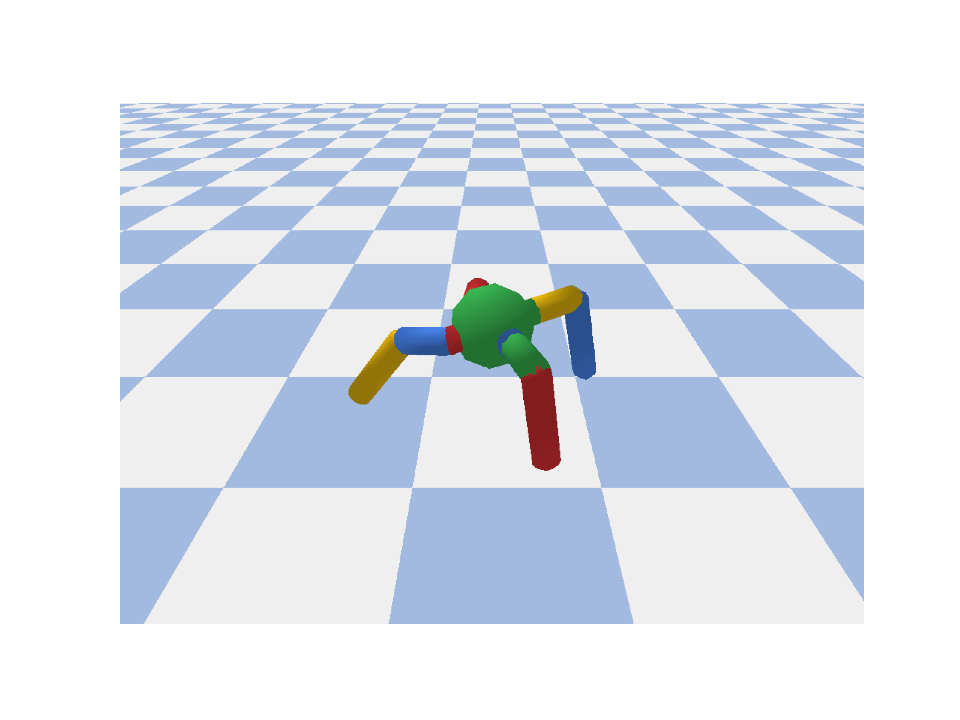
\includegraphics[width=0.45\textwidth]{damaged_robot.pdf}
\caption{The robot walking with one leg (left blue-yellow leg) damaged.
The knee flexion angle of this leg is fixed at $30^{\circ}$ to reduce contact with the ground.
}
\label{damaged_robot}
\end{figure}




\subsection{Generating the Repertoire with MAP-Elites}
To implement MAP-Elites, the task space for our robot is defined to be its 2D displacement, spanning from -4.8 to 4.8 on both the $x$ and $y$ axes. 
This continuous space is then discretized into a $32 \times 32$ grid, yielding a resolution of 0.3 unit per cell.
In each iteration of MAP-Elites, we generate 128 off-springs from 8 selected parents using a specially designed crossover operation.
We then evaluate these off-springs to obtain their outcomes and fitnesses. 
To evaluate each genotype, we first decode it into the periodic targets and then execute them for 4 seconds in simulation.
We used default simulation settings for evaluation, where we set the friction coefficient equal to $1.0$ with no damage and no payload (full torque).
Note that, while evaluating each off-spring, we need to record the 2D displacement as well as the three parameters in arc-based dynamics representation.
These data will be used as the baseline for the dynamics in the following steps. 
The fitness is defined to be a reward of the lifespan (number of time-steps before the body of the robot hits the ground) penalized by the electrical cost \cite{QDgym}.
We run the MAP-Elites for 4000 iterations, and obtained 753 elementary policies (see Fig. \ref{original_repertoire}).
To speed up the process, we used 10 CPU cores to conduct the evaluation of the off-springs in parallel.


In our crossover operation, we implemented three types of mutations.
The first one leverages the design of the Ant robot that its motion is powered by the four legs acting independently.
Since each motor is controlled by three parameters, each leg of the Ant robot can be fully described by 6 parameters which can be regarded as the gene segment for this leg.
In this type of mutation, each leg has 20\% chance to use the corresponding gene segment from another controller (another parent).
Thus, we allow the gene segments to be swapped between parent controllers, generating new genotypes with different combinations of leg motions.
This ensures good inheritance from the parents, which may potentially give birth to new motions of high quality.
The second type is large mutation for exploration.
Since we cannot expand our gene pool by simply swapping the gene segments, we use the similar design in \cite{cully2015robots} that each parameter has 10\% of probability to mutate into any possible value. 
This large mutation ensures good exploration of new genotypes and may effectively overcome local optimum.
Considering large mutation may harm inheritance, we apply this large mutation to only 60\% of off-springs.
The third mutation is adding small noises to help with local search.
There are $55.21\%$ of the off-springs that experienced large mutation and $59.04\%$ that have swapped leg gene segments.
For the remaining $18.34\%$ of off-springs that experienced neither these two mutations, adding this small noise acts as a fine-tuning mechanism.
Hence, we designed a crossover operation that achieves good exploitation via inheritance and ensures sufficient exploration by introducing large mutation for global search and fine-tuning for local search. 
The pseudo code for our crossover operation is shown below.


\begin{algorithm}
\caption{Crossover}
\begin{algorithmic}
\STATE \textbf{procedure} Crossover
\STATE \textbf{input} parent genotypes $\mathcal{G}$, batch size $N$
\STATE $\mathcal{R} \leftarrow \emptyset$ \COMMENT{Initialize off-springs}
\FOR{$\bm{i} = 1 \rightarrow N$}
\STATE \# 20\% chance for each leg to use swapped gene
\STATE $\theta_i \leftarrow $ swap{\_}leg{\_}genes($\mathcal{G}$, 0.2)
\STATE $\mathcal{R}$.append($\theta_i$)
\ENDFOR

\STATE  \COMMENT{Applies to 60\% of off-springs}
\FOR{$\bm{i} = 1 \rightarrow N$}
\IF{random{\_}number < 0.6} 
\STATE $\theta_i \leftarrow \mathcal{R}$[$i$] 
\STATE \# 10\% chance of large mutation for each parameter 
\STATE $\theta'_i \leftarrow$ large{\_}mutation($\theta_i$, 0.1)
\STATE $\mathcal{R}$[$i$] $\leftarrow \theta'_i$
\ENDIF
\ENDFOR

\STATE  \COMMENT{Add small noises to all off-springs}
\FOR{$\bm{i} = 1 \rightarrow N$}
\STATE $\delta_i \leftarrow \mathcal{N}(0, 0.1)$
\STATE $\mathcal{R}$[$i$] $\leftarrow$ clip($\mathcal{R}$[$i$] + $\delta_i$, 0, 1)
\ENDFOR

\RETURN $\mathcal{R}$
\end{algorithmic}
\label{Crossover}
\end{algorithm}


\begin{figure}[h]
\centering
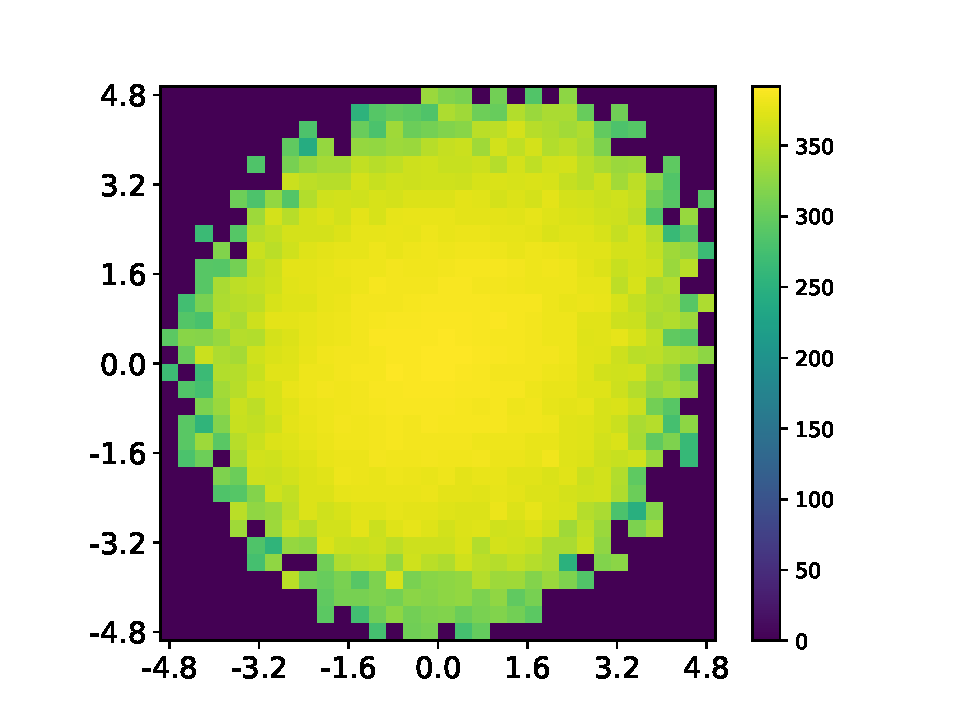
\includegraphics[width=0.45\textwidth]{original_map_elites.pdf}
\caption{The resultant repertoire after 4000 MAP-Elites iterations.
The coordinates correspond to the 2D displacement brought by each policy, and the color indicates the fitness score.
Policies leading to smaller displacements have bigger fitnesses as they require lesser electric cost.
}
\label{original_repertoire}
\end{figure}









\subsection{Determine the Coordinates of Policies}
After having generated the repertoire, we can evaluate the policies in different simulation settings to get the distortion basis.
These basis will then follow a dimensional reduction via SVD and finally converted into the coordinate system using PCA transform.
To prepare a wide range of environments to collect distortions, we selected 6 environments for each damage condition (intact case and four damaged cases for four legs), where the friction and torque ratio (to model payload) for each environment are randomly selected from a uniformly distribution between 0.7 to 1.
Thus, we acquired 30 different environments in total.
We then evaluate the entire repertoire in each one of the environments and record the dynamics representations for each policy.
There are two different representations of dynamics used in this paper, displacement-based and arc-based (see Fig \ref{baseline_trajectories}). 
The distortion is defined to be actual outcome minus the baseline, where our baselines are the dynamics representations recorded during the MAP-Elites evaluations.
The distortion for the direction $\varphi$ in arc-base representation is rather special due to the periodic nature of angles.
For example, if the baseline direction is $30^{\circ}$ and actual outcome is $330^{\circ}$, the distortion should be $-60^{\circ}$ instead of $300^{\circ}$.
Hence, we need to make sure that the directional distortion always lies between $-180^{\circ}$ to $180^{\circ}$.

\begin{figure}[h]
\centering
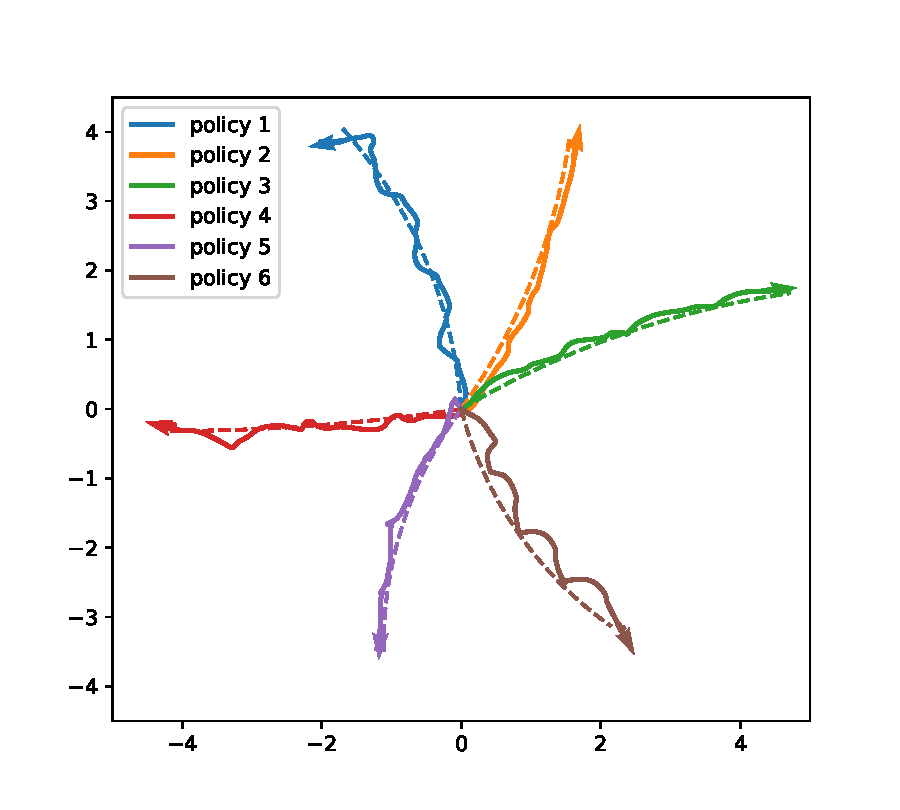
\includegraphics[width=0.45\textwidth]{original_trajectories_1.pdf}
\caption{The trajectories of 6 elementary policies in default simulation settings.
The dashed lines denote the predicted trajectories in arc-based representation with the parameters calculated using Eq. (\ref{all_three_parameters}).
The fact that the predicted curves stick closely to the actual trajectories indicates such representation being successful.
}
\label{baseline_trajectories}
\end{figure}


We then use the results to conduct dimensionality reduction via SVD.
For displacement-based representation, this is easy to achieve.
However, this is not applicable for arc-based representations since the measurement noises are different for different policies.
Hence, we take an alternative approach by finding the basis that minimizes the squared distance error.
This is inspired by the fact that regular dimensionality reduction via SVD is essentially minimizing the squared reconstruction error.
For displacement-based representation, minimizing the squared error for $x$ and $y$ displacements is equivalent to minimizing the squared distance error. 
To do this for arc-based representation, we know that the reconstructed distortion matrix can be expressed in the following form:
\begin{equation}
\begin{gathered}
%
\hat{\bm{A}} = \bm{A} \bm{U} \bm{P}
%
\end{gathered}
\label{SVD_for_arc}
\end{equation}
where $\bm{A}$ is the original distortion matrix of size $N \times n$, $\bm{U}$ is a $n \times s$ matrix, and $\bm{P}$ is a $s \times n$ matrix.
Matrix $\bm{A} \bm{U}$ gives the linear basis we are looking for, and matrix $\bm{P}$ reconstructs the original matrix from the basis.
This applies to all three parameters in arc-based representation, and we can calculate the predicted displacement from the reconstructed distortion matrix using Eq. (\ref{position_from_arc}).
Note that the matrix $\hat{\bm{A}}$ is the distortion, hence to recover the predicted parameters we need to add the baseline results.
To minimizes the squared error in distance, we used gradient descend to update the $\bm{U}$ and $\bm{P}$ matrix for each parameter.
This requires the initial values for the $\bm{U}$ and $\bm{P}$ matrix, which can be the ones found in SVD.
Hence, the initial $\bm{U}$ matrix is the same as in Eq. (\ref{ATA}), and the initial $\bm{P}$ matrix is $\bm{U}^T$.
We then ran the gradient descent for 2000 iterations with a learning rate of $0.0005$, and we finally took the $\bm{A} \bm{U}$ matrix as our basis.


To determine the number of dimensions we need, we plotted out the error against the dimension number in Fig \ref{original_elbow}.
We then used elbow method \cite{elbow} to determine the dimension number to be 5.
However, we can see from this plot that the remaining error is still quite large especially for arc-based representation.
A deeper investigation tells that this is because some policies are very noisy, and their outcomes seem to be not predictable.
Hence, we filter out the policies with squared errors larger than 3.
This leaves us with 398 remaining policies, and we replotted the curve in Fig \ref{filtered_elbow}.
We can see that the elbow is still at 5 while the error is greatly reduced.
The two curves also become closer, although the remaining error for arc-based representation is still larger.
To check that our filtering does not harm the coverage of the repertoire, we plotted out the remaining polices in task space (see Fig \ref{filtered_repertoire}).
We can see that our filtering does create some vacancies, but overall the task space is still well covered.
Finally, we use PCA transform to convert the basis into the coordinates in the input space.


\begin{figure}[h]
\centering
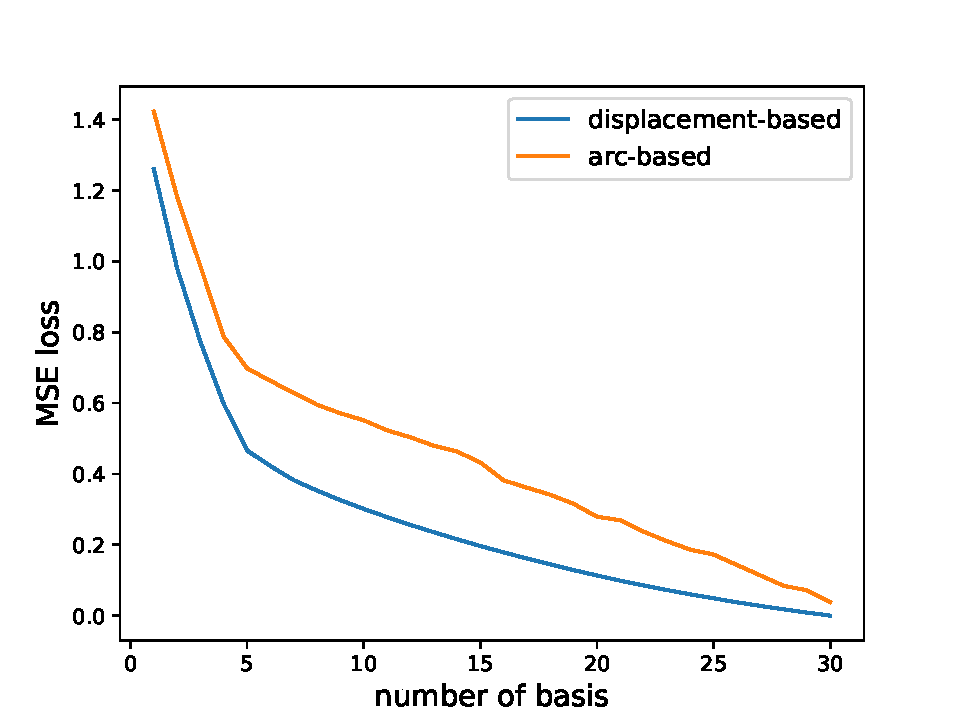
\includegraphics[width=0.45\textwidth]{elbow.pdf}
\caption{The mean squared distance error against the number of basis.
The elbows for the two curves are both at 5.  
}
\label{original_elbow}
\end{figure}


\begin{figure}[h]
\centering
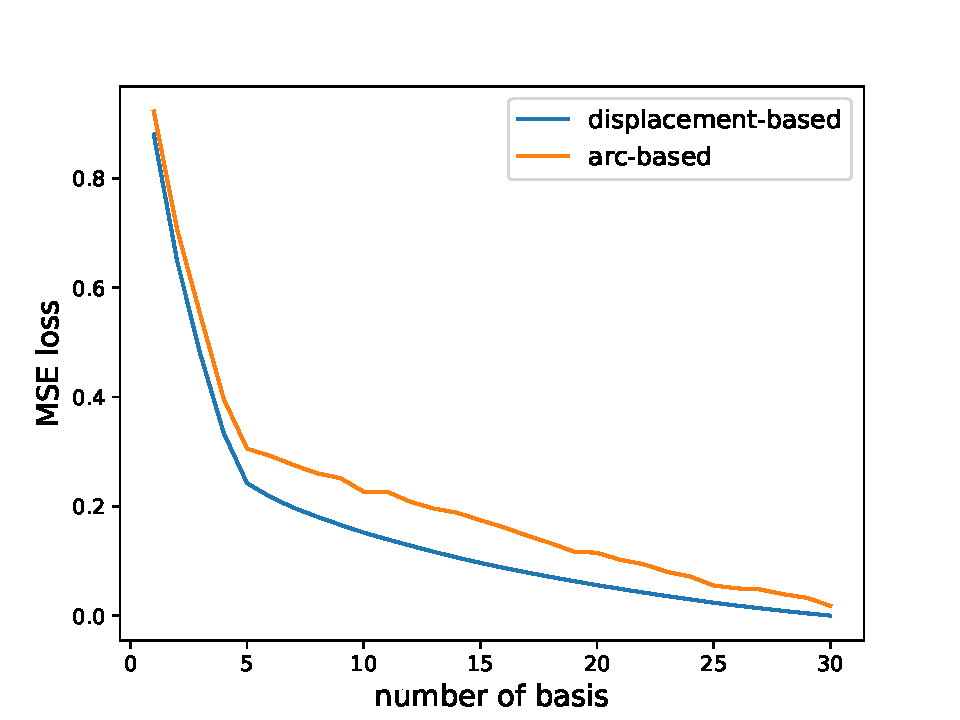
\includegraphics[width=0.45\textwidth]{filtered_elbow.pdf}
\caption{The mean squared distance error against the number of basis after filtering out the policies with large errors.
}
\label{filtered_elbow}
\end{figure}

\begin{figure}[h]
\centering
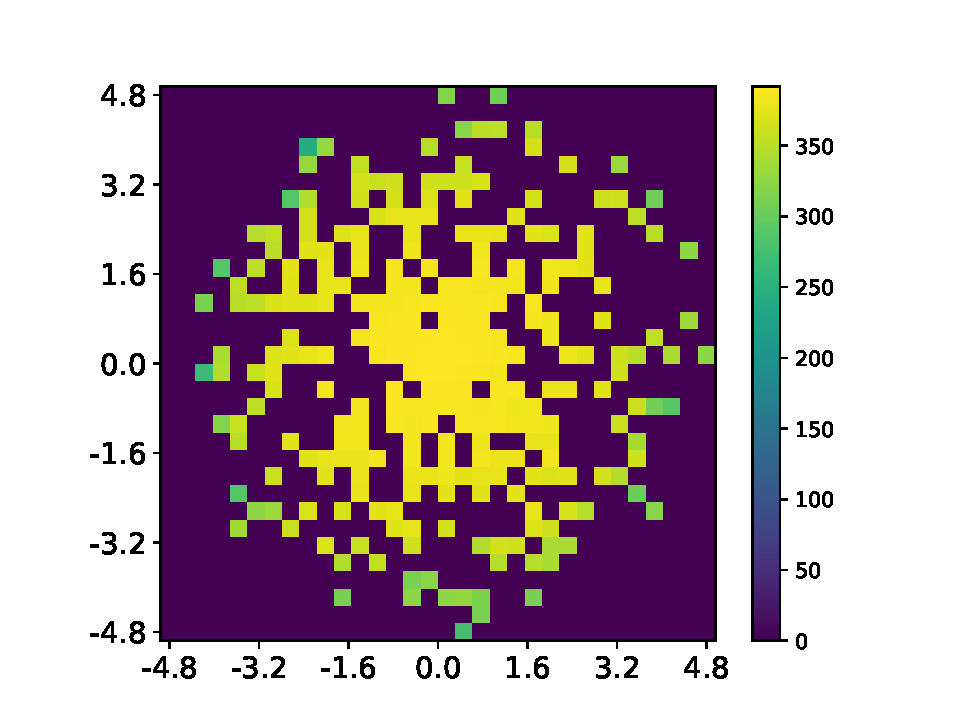
\includegraphics[width=0.45\textwidth]{filtered_map_elites.pdf}
\caption{The remaining repertoire after filtering.
}
\label{filtered_repertoire}
\end{figure}







\subsection{Clustering the Collaboratively Collected Data}
We can then evaluate our collaborative learning algorithm by clustering some collaboratively collected data and testing the adaptation performance. 
First, we need to conduct the Monte Carlo sampling required by DP clustering.
To do this, we randomly sampled 128 environments with 64 interaction data for each environment.
The damage status of these environments is evenly distributed for five damage conditions, and the friction and the torque are both uniformly distributed from 0.7 to 1.
The model parameters for each sample are determined with MLE.
One thing to notice is that, although our kernel should be Matern $\frac{5}{2}$ since we have assumed the dynamics to twice differentiable when deriving the linear prior mean function, it is found that Matern $\frac{3}{2}$ fits better to our data.
This is likely because the noises are also incorporated in the basis of our prior mean function, which harms the smoothness of the residual.
After having determined the priors of model parameters, we can test our clustering method on real-world data.
However, the collection of real-world data is too expensive for this project, hence we simulated this by randomly sampling a few episodes of data from several simulated environments.
The details about these environments can be found in Table \ref{data}.
Since we do not require the data to come from the same environment, we add a small noise to the environment parameters each time we sample an episode.
Considering the fact that the length of the episodes are not necessarily consistent, the length of each episode randomly fluctuates from 6 to 20.
We then performed 200 Gibbs sweeps to identify the configuration of cluster assignment with the largest posterior likelihood.
During clustering, the concentration parameter $\alpha$ is 1, and the threshold of the data size to apply posterior convergence is set to 30.

\begin{table}
\caption{Collaboratively Collected Data}
\centering
\def\arraystretch{1.2}
\begin{tabular}{|c||c|c|c|c|}
\hline
Label & env 1 & env 2 & env 3 & env 4\\
\hline
Damage & intact & leg 1 & leg 2 & leg 3 \\
\hline
Friction & 0.95 $\pm$ 0.01 & 0.85 $\pm$ 0.01 & 0.73 $\pm$ 0.01 & 0.88 $\pm$ 0.01 \\
\hline
Torque & 0.95 $\pm$ 0.01 & 0.92 $\pm$ 0.01 & 0.90 $\pm$ 0.01 & 0.76 $\pm$ 0.01 \\
\hline
Amount & 20 & 10 & 5 & 15 \\
\hline
\end{tabular}
\label{data}
\end{table}



\subsection{Model-Based Adaptation in a Maze}
To test the adaptation performance, we deployed our robot in a maze (see Fig \ref{maze}) with unknown dynamics and let it navigate to the exit as fast as possible.
The robot knows its position and orientation at each time-step, but the outcomes of executing each policy need to be learned online.
The radius of the robot is 0.41.
If the distance to the closest obstacle is smaller than this value, the robot collides with the obstacle.
In this case, the robot will spend another time-step to return to its previous position.
Hence, having collision will waste two time-steps, but the robot can acquire the outcome of the policy that led to the collision.



To perform model-based adaptation, the robot uses a simple planning algorithm similar to the dynamic window approach \cite{DWA}.
In every time-step, the repertoire stands for all the possible actions that the robot can take.
The outcomes of those actions are predicted using the learned model.
These predicted outcomes are then evaluated by an objective function:
\begin{equation}
\begin{gathered}
G(\bm{s}, \hat{\bm{s}}') = \operatorname{heading}(\hat{\bm{s}}') - 
\operatorname{penalty}(\operatorname{dist}(\hat{\bm{s}}')) \\
- k \cdot \operatorname{collision}(\bm{s}, \hat{\bm{s}}')
\end{gathered}
\label{objective_function}
\end{equation}
where $\bm{s}$ denotes the current state of the robot, and $\hat{\bm{s}}'$ stands for the predicted subsequent state by executing the elementary policy.
The term $\operatorname{heading}(\hat{\bm{s}}')$ quantifies the alignment of the action with the target, and the $\operatorname{penalty}(\operatorname{dist}(\hat{\bm{s}}'))$ term penalizes the distance to the closest obstacle.
The last term $\operatorname{collision}(\bm{s}, \hat{\bm{s}}')$ is a binary function that returns $1$ if transition $\bm{s} \rightarrow \hat{\bm{s}}'$ leads to collision and $0$ otherwise.
$k$ is a large positive value to give a large penalty for collision.
The robot uses this objective function to evaluate all the elementary policies and executes the one with the highest result.
After execution, the robot updates its state $\bm{s}$ as well as the dynamics model before taking the next step.
This process is repeated until the robot reaches the exit or runs out of time.



In our implementation, the state $\bm{s}$ refers to the position of the robot. 
The dynamics model predicts the 2D displacement for each policy, which is then converted into the subsequent state $\hat{\bm{s}}'$ using the following formula:
\begin{equation}
\hat{\bm{s}}' = \bm{s} + 
\begin{bmatrix}
\cos (\theta) & -\sin(\theta) \\
\sin (\theta) & \cos(\theta) \\
\end{bmatrix}
%
\begin{bmatrix}
\Delta \hat{x} \\
\Delta \hat{y} \\
\end{bmatrix}
\label{predicted_subsequent_state}
\end{equation}
where the $\theta$ is the orientation of the robot.
For arc-based dynamics representation, the predictions need to be transformed into displacement using Eq. (\ref{position_from_arc}).
There is a problem that the predicted outcome given by Eq. (\ref{simplified_distortion}) is not a value but a mixture of Gaussian distributions.
For simplicity, we just used the mean as the predicted result, which is a linear combination of the means for each Gaussian:
\begin{equation}
\begin{gathered}
\hat{x}^*_d 
= \sum_j p(c=j| \bm{x}_{1:N}) \mu(x^*_d|\bm{\theta}^*_j, \bm{x}_{1:N})
\\
+ \,\, p(c \neq j, \forall j|\bm{x}_{1:N})  \mu(x^*_d|\bm{x}_{1:N}, \text{RTE})
\end{gathered}
\label{predicted_mean}
\end{equation}
In practice, it is found that the RBF kernel used in the original RTE method \cite{RTE} severely overestimates the smoothness.
As a result, we used Matern $\frac{1}{2}$ with prior variance set to $4$ instead.
The $\operatorname{heading}(\hat{\bm{s}}')$ term in the objective function is defined to be the effective travelled distance, which is the projection on the suggested path.
The distance penalty is a specially designed function:
\begin{equation}
\begin{gathered}
\operatorname{penalty}(x) = \frac{0.162}{(x - 0.23)^2}
\end{gathered}
\label{penalty}
\end{equation}
Such design is to satisfy two important properties.
First, $\frac{d}{d x} (\operatorname{penalty})|_{(0.41 + 0.5)} \approx -1$.
Since $|\nabla(\operatorname{heading})| \leq 1$, this suggests that the sum of the first two terms in $G(\bm{s}, \hat{\bm{s}}')$ is sure to decrease when the distance is smaller than $0.5 + 0.41$.
Hence, we have inexplicitly defined the safe distance to be 0.5 to account for the uncertainties in model predictions.
The second property is that $\operatorname{penalty}(0.41) = 5$. 
This means that when the robot is about to collide, the penality will exceed the maximum increase in $\operatorname{heading}$ that can happen in one time-step, which is 4.8.
Finally, coefficient $k$ in the last term is set to 100.




 



\begin{figure}[h]
\centering
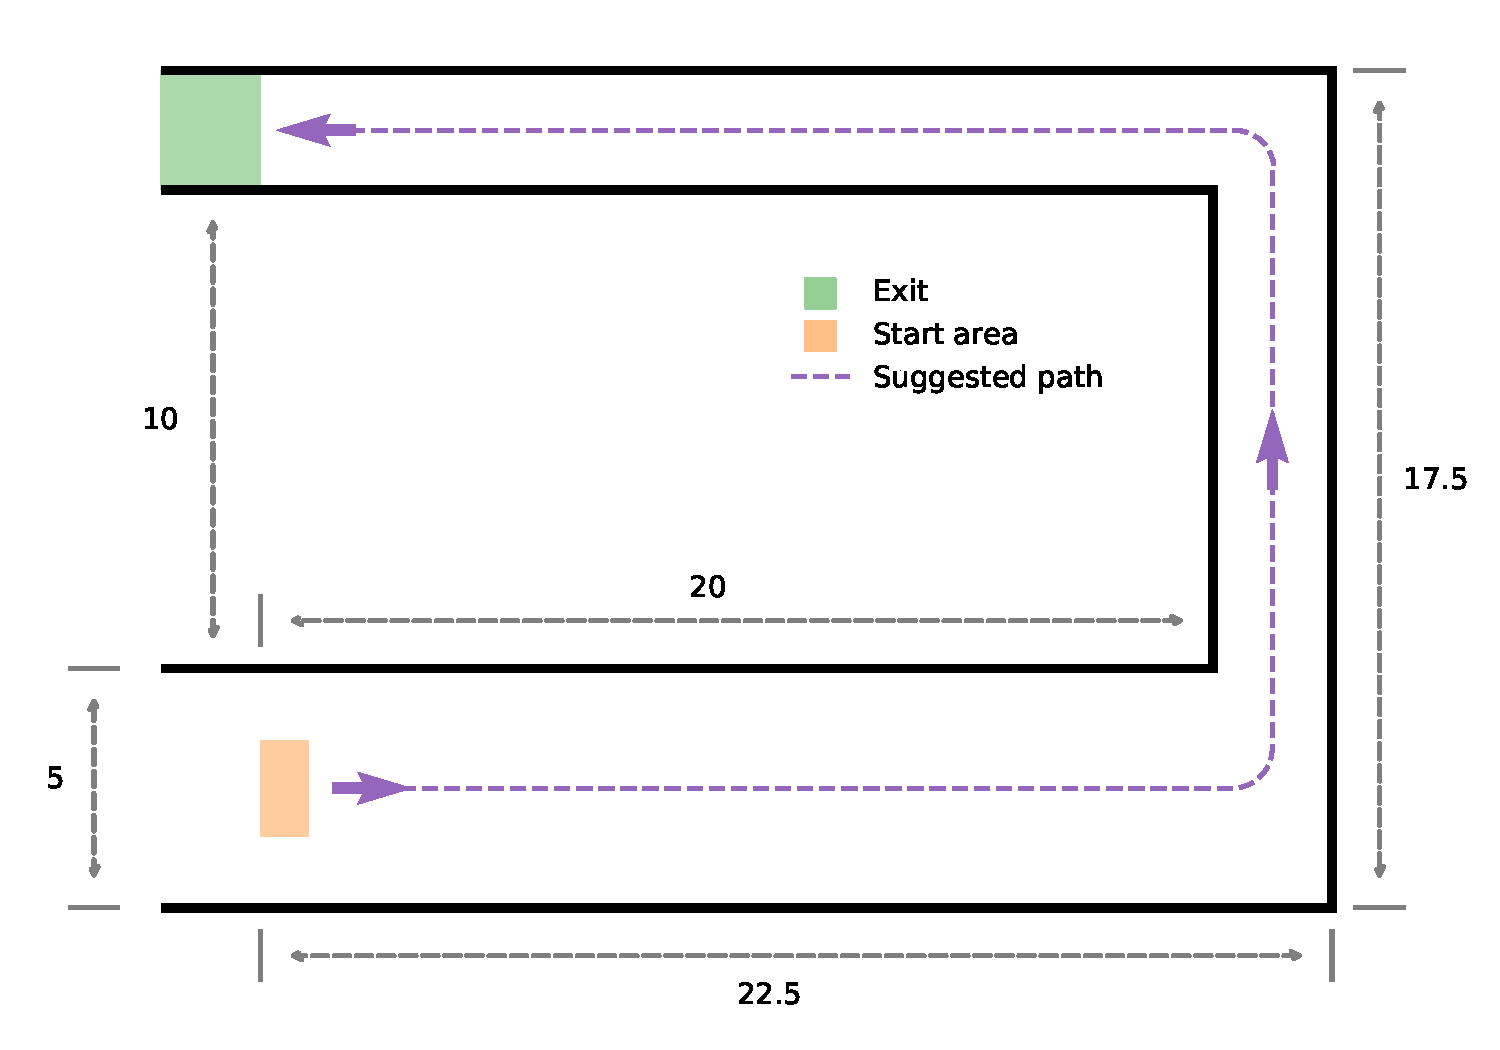
\includegraphics[width=0.45\textwidth]{tunnel_floorplan.pdf}
\caption{The floor-plan of the maze.
The starting area is a rectangle with width equals to 1 and height equals to 2.
To allow some exploration at start, the width of the tunnel is 5 before the first turning and then reduces to 2.5 for the rest of the sections.
}
\label{maze}
\end{figure}





